\documentclass{article}
\setlength{\parskip}{5pt} % esp. entre parrafos
\setlength{\parindent}{0pt} % esp. al inicio de un parrafo
\usepackage{amsmath} % mates
\usepackage[sort&compress,numbers]{natbib} % referencias
\usepackage{url} % que las URLs se vean lindos
\usepackage[top=25mm,left=20mm,right=20mm,bottom=25mm]{geometry} % margenes
\usepackage{hyperref} % ligas de URLs
\usepackage{graphicx} % poner figuras
\usepackage[spanish]{babel} % otros idiomas
\usepackage[utf8]{inputenc}
\author{Equipo 4 \\Jorge  Fuentes, Tania  Hernandez,
 Anahi Herrera, Gustavo  Díaz, Miriam  Mata, Alejandro Ramos} % author
\title{Práctica 1 \\ Optimización topológica con MATLAB} % titulo
\date{\today}

\begin{document} % inicia contenido
\maketitle % cabecera
\begin{abstract} % resumen
 \textbf{Objetivo:} El estudiante conocerá cada una de las secciones que integran el código de optimización topológica, como se debe crear un archivo (.m) en MATLAB y cómo se ejecuta el análisis.\\
 La optimización de la topología comenzó en 1904 con las estructuras de Michell. Aquí, Michell consideró las estructuras de vigas y también desarrolló una teoría de diseño según la cual todas las estructuras de vigas se cruzan entre sí en un ángulo de 90°. En consecuencia, se creó una disposición óptima de los esfuerzos de tracción y compresión.Una vez mencionado esto hablemos sobre lo que estaremos trabajando, el código a utilizar se le llama código de optimización de topología de 99 líneas, en la que se presenta una cantidad de 99 líneas de código en Matlab en la que las 99 líneas de entrada corresponden al optimizador y a la subrutina de elemento finito, El código de 99 líneas se divide en varias estructuras que componen cada una a cierta parte del programa que realiza cierta acción. De las 99 líneas de código: 36 líneas pertenecen al programa principal 12 líneas pertenecen a criterio optimizador 16 líneas a la independencia de mallado y 35 líneas al código de elemento finito Viendo el código sin líneas de comentarios obtenemos que con tan solo 19 líneas de código son realmente Necesarias para hacer dicha optimización de geometrías. Agregando 3 líneas más de códigos seremos capaces de agregar múltiples cargas. Donde lo implementaremos en MATLAB que es un programa muy potente con el cual podremos realizar cálculos numéricos con vectores y matrices, trabajar con números escalares, tanto reales como complejos y utilizar una amplia variedad de gráficos en dos y tres dimensiones. MATLAB tiene un lenguaje propio de programación, El lenguaje de cálculo técnico desarrollado por MathWorks, es un entorno de programación para el desarrollo de algoritmos, análisis de datos, visualización y cálculo numérico.
\end{abstract}
\newpage
\tableofcontents
\section{Introducción}\label{intro} % seccion y etiqueta
En esta práctica se estará realizando el código de optimización topológica de 99 líneas se divide en 36 líneas para la programación principal, 12 líneas para los criterios de optimización, 16 líneas para el filtro de mallado y 35 líneas para el código de elemento finito. De hecho, excluyendo las líneas de comentarios y líneas asociadas con la producción y el análisis de elementos finitos, el código resultante es de solo 49 líneas.
Para poder llevar a cabo la práctica se tuvo que realizar una investigación grupal para poder entender la metodología y para poder llegar a una implementación exitosa en el programa de MATLAB. Las evidencias de lo mismo se anexarán más adelante. 

%\cite{ff2} CITAR FUENTE

%\begin{figure} % figura
    %\centering
    %\includegraphics[width=150mm]{output3.jpg} % archivo
    %\caption{resultados del programa}
    %\label{grafica}
%\end{figure}
\newpage
\section{Desarrollo}
\subsection{Nombre y definición de la programación}
\subsubsection{Sobre MATLAB}
Es un programa muy potente con el cual podremos realizar cálculos numéricos con vectores y matrices, trabajar con números escalares, tanto reales como complejos y utilizar una amplia variedad de gráficos en dos y tres dimensiones. MATLAB tiene un lenguaje propio de programación, El lenguaje de cálculo técnico desarrollado por MathWorks, es un entorno de programación para el desarrollo de algoritmos, análisis de datos, visualización y cálculo numérico\cite{rf1}.
\subsubsection{La Optimización topológica}
La optimización topológica es una técnica englobada dentro del campo de análisis estructural. Se basa en el análisis mecánico de un componente o estructura. Su principal objetivo es el aligeramiento estructural manteniendo las funcionalidades mecánicas del componente objetivo\cite{rf2}. A diferencia de otros tipos de optimización, la optimización topológica ofrece un nuevo concepto de diseño estructural enfocado a aquellas aplicaciones donde el peso del componente es crucial (por ejemplo, la industria aeroespacial).
\subsubsection{Hablemos del Código de 99 líneas}
Se le llama código de optimización de topología de 99 líneas, en la que se presenta una cantidad de 99 líneas de código en Matlab en la que las 99 líneas de entrada corresponden al optimizador y a la subrutina de elemento finito, El código de 99 líneas se divide en varias estructuras que componen cada una a cierta parte del programa que realiza cierta acción\cite{rf3}. De las 99 líneas de código: 36 líneas pertenecen al programa principal 12 líneas pertenecen a criterio optimizador 16 líneas a la independencia de mallado y 35 líneas al código de elemento finito Viendo el código sin líneas de comentarios obtenemos que con tan solo 19 líneas de código son realmente Necesarias para hacer dicha optimización de geometrías. Agregando 3 líneas más de códigos seremos capaces de agregar múltiples cargas.
\subsection{Estado del arte}
La optimización de la topología comenzó en 1904 con las estructuras de Michell. Aquí, Michell consideró las estructuras de vigas y también desarrolló una teoría de diseño según la cual todas las estructuras de vigas se cruzan entre sí en un ángulo de 90°. En consecuencia, se creó una disposición óptima de los esfuerzos de tracción y compresión. \\
Además, hoy en día también es un método de desarrollo de productos asistido por ordenador con el que se puede reconocer el potencial de optimización en una fase temprana del proceso de desarrollo. Por ello, varios proveedores de software ofrecen hoy en día soluciones para ello. \\
\subsubsection{Ventajas que ofrece la optimización de la topología}
Dependiendo de la aplicación, hay casi una multitud de objetivos. Sin embargo, el objetivo fundamental es aprovechar al máximo el espacio de la instalación.
También otros ejemplos son estos: 
\begin{itemize}
  \item Reducción de peso con una capacidad de carga invariable
  \item	Aumento de la carga con un peso constante 
  \item Optimización de la distribución de la fuerza en varios puntos de apoyo \item Optimización de la frecuencia natural mediante la relación correcta de       masa y rigidez
\end{itemize}
\subsubsection{Tipos de optimización de la topología existentes}
En resumen, la optimización topológica se ocupa de encontrar la forma básica (topología) más favorable para los componentes con carga mecánica. En este contexto, se distingue entre optimización continua y discreta, además de los ámbitos de aplicación y los objetivos de optimización descritos anteriormente.
\subsubsection{Optimización discreta}
El representante más conocido es Anthony George Maldon Michell y su personal trabaja. Estas optimizaciones por trabajos de barra se siguen utilizando hoy en día, ya que las ventajas residen principalmente en el bajo tiempo de cálculo. 
\subsubsection{Optimización continua}
Para ello, el proceso se realiza generalmente en 3 pasos, a saber.\\
Hay que definir el espacio máximo de instalación disponible. De esta manera dEsto puede hacerse mediante CAD o un sistema de elementos finitos.
Es necesario establecer otros objetivos de optimización, como: de baja masa o alta rigidez.\\
El software utiliza los datos disponibles para determinar uno o más Propuestas de diseño que sirven de plantilla para el concepto de diseño del diseñador. está disponible para su uso.\\
Estaremos encantados de asesorarle sobre cómo puede mejorar y, sobre todo, acelerar su proceso de desarrollo de productos con la ayuda de la optimización topológica.
\newpage
\subsection{Procedimiento de la programación}
A continuación, veremos la codificación de la programación en MATLAB.
\begin{figure}[htp] % figura
    \centering
    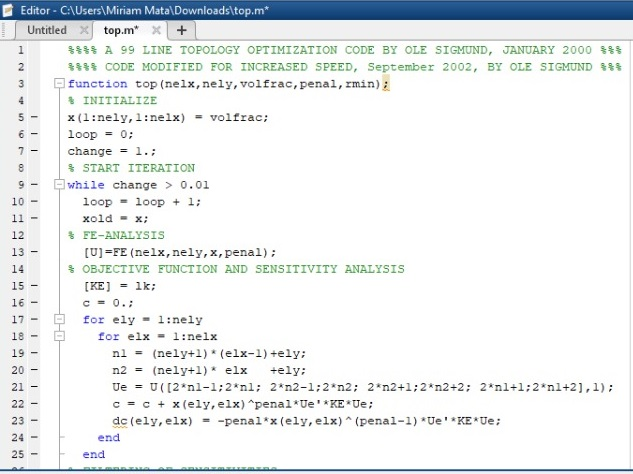
\includegraphics[width=140mm]{Codigo 1.jpeg} % archivo
    \caption{Configuraciones iniciales y análisis de sensibilidad.}
    \label{grafica}
\end{figure}
\begin{figure}[htp] % figura
    \centering
    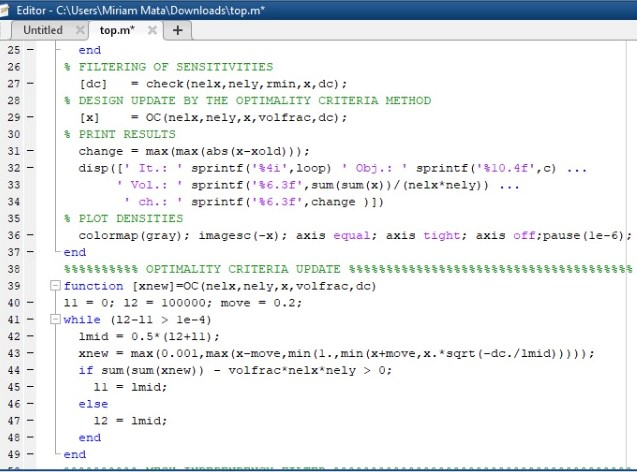
\includegraphics[width=140mm]{Codigo 2.jpeg} % archivo
    \caption{Optimización e impresión de resultados.}
    \label{grafica}
\end{figure}
\begin{figure}[htp] % figura
    \centering
    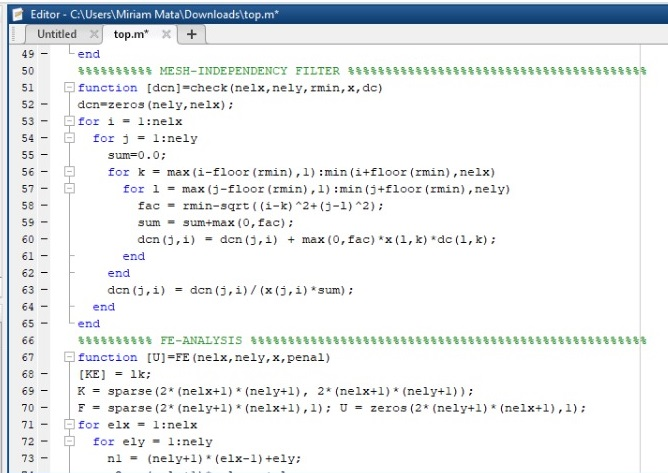
\includegraphics[width=140mm]{Codigo 3.jpeg} % archivo
    \caption{Filtro de independencia - Mesh.}
    \label{grafica}
\end{figure}
\begin{figure}[htp] % figura
    \centering
    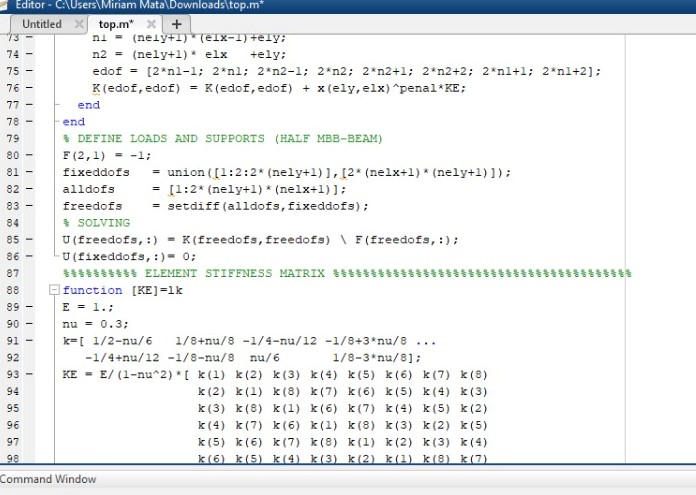
\includegraphics[width=140mm]{Codigo 4.jpeg} % archivo
    \caption{Matriz de rigidez del elemento.}
    \label{grafica}
\end{figure}
\newpage
\subsection{Implementación de la programación}
\begin{figure}[htp]
 \centering
   { 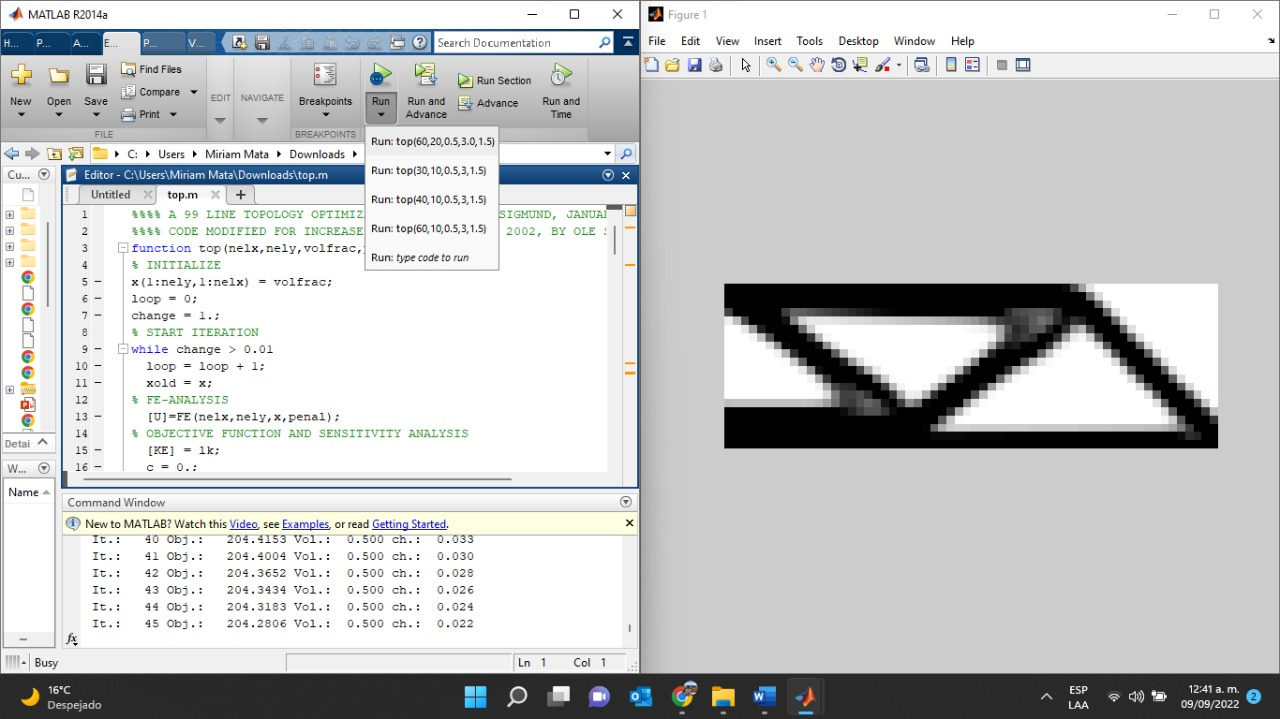
\includegraphics[width=1\textwidth]{Optimizar.jpeg}}
   {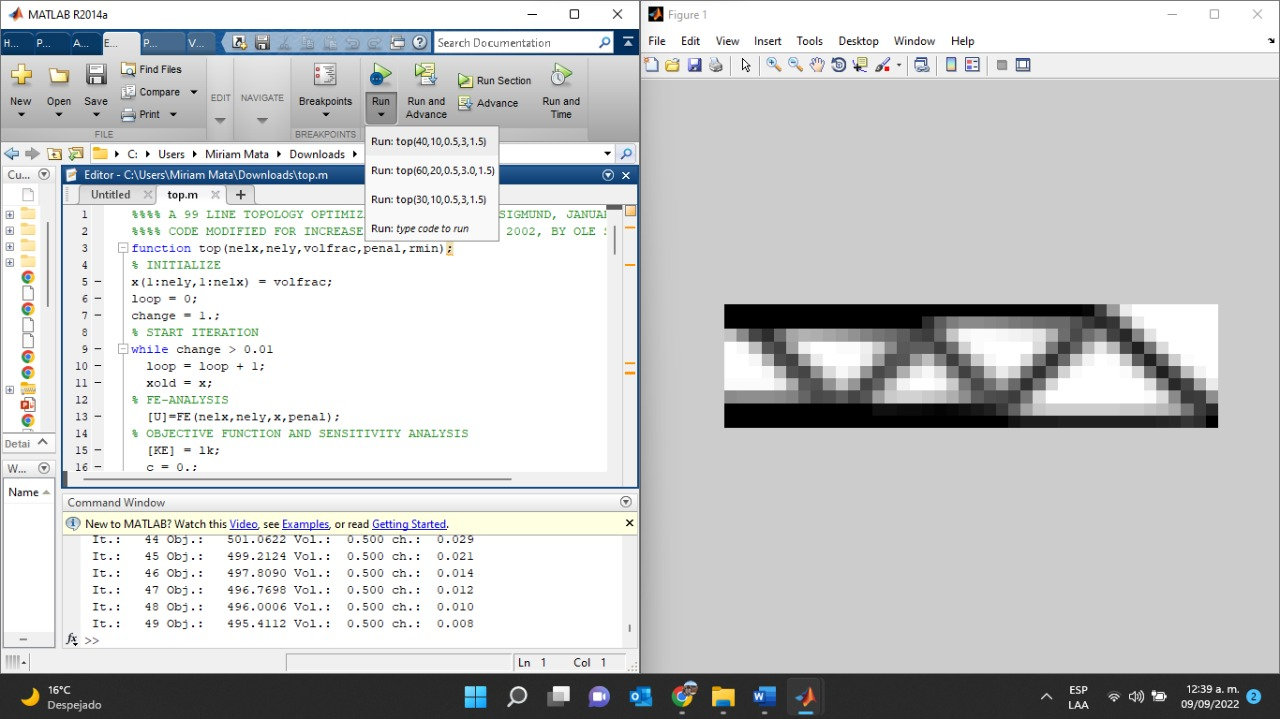
\includegraphics[width=1\textwidth]{Optimizacion.jpeg}}
     \caption{Resultados de la Optimización topológica 1.}
\end{figure}
   
\begin{figure}[htp]
\centering
   { 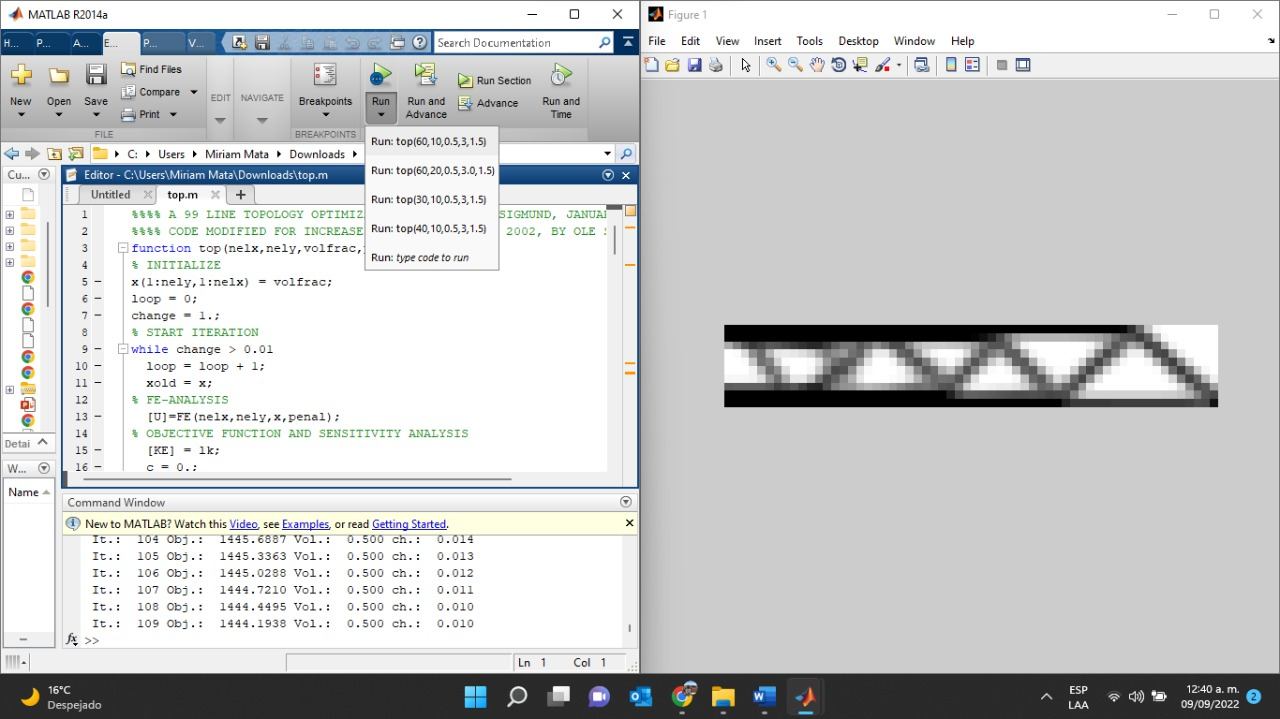
\includegraphics[width=1\textwidth]{Optimizar 2.jpeg}}
    {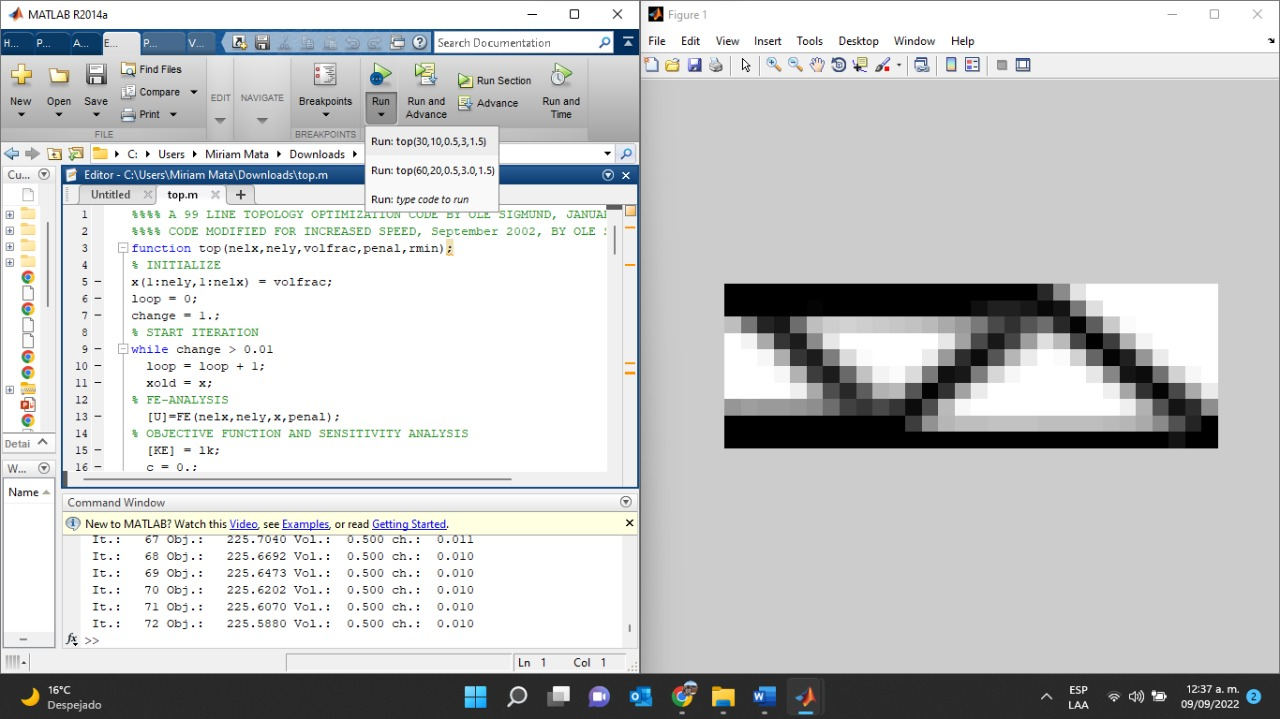
\includegraphics[width=1\textwidth]{Optimizacion 2.jpeg}}
  \caption{Resultados de la Optimización topológica 2.}
\end{figure}
   
 \newpage
\section{Conclusiones}
\subsection{Jorge  Fuentes}
Trabajar nuevamente con MATLAB fue una sorpresa para mí, no recordaba mucho de como utilizar dicha herramienta de simulación de matrices por lo que me costó un poco entender sobre que estaba haciendo exactamente el código utilizado en nuestra práctica. Una vez entendido fue fácil modificar las variables para ver los resultados que mostraba la optimización de la topología de los elementos que estábamos usando. La ejecución del análisis así como se hace el código en MATLAB fueron de gran ayuda para repasar la programación, ya que, como sabemos la optimización topológica va de la mano con la biomecánica al momento de optimizar los elementos a un grado óptimo y funcional.
\subsection{Tania  Hernandez}
La practica se enfoco en la programacion de matlab, como forma del proceso que con lleva el programar en el mencionado programa, especificamente de un codigo extenso, asi como tambien en el estado del arte de la pieza elaborada, ya que todo lo investigado, nos fue util para la realizacion de la pieza.
\subsection{Anahi Herrera}
Gracias a la elaboración de esta práctica se entendió de una mejor manera el funcionamiento de MATLAB aplicado hacia la materia de biomecánica, se realizaron investigaciones grupales llevando esta teoría recopilada a la práctica de manera exitosa. 
\subsection{Gustavo  Díaz}
Durante el desarrollo de esta practica vimos el funcionamiento de cierto programa dentro del software de Matlab en el cual se nos pidió hacer un modelado de una viga dentro de la optimización topológica y así poder hacer el diseño de la pieza de manera rápida y eficiente esta simulación se hace con la intención de optimizar la menor cantidad de material o tiempo requerido para realizarla pero sin deformarse, hacerlo en Matlab ayuda dado que puedes hacer el diseño de la pieza y ver cada uno de los análisis de las piezas.
\subsection{Miriam  Mata}
Esta práctica estuvo muy interesante porque a pesar de ya haber de usar Matlab en semestres anteriores en lo personal nunca había usado un código como este, fue un poco complicado, pero se logró, siento que a nosotros como futuros ingenieros en mecatrónica se nos debió de haber inculcado más la programación desde los primeros semestres, ya que si bien la mayoría se va a el área de diseño en cierta parte seguimos viendo programación, pero esta actividad me ayudo para poder refrescar un poco mis conocimientos en Matlab porque en sí es un compilador muy sencillo de usar también depende mucho de la librería que te sepas por qué va cambiando cada año.
\subsection{Alejandro Ramos}
En esta práctica lo que vimos más que nada fue la teoría, y la programación esto nos viene muy bien para ir agarrando las bases o los fundamentos para que en las siguientes prácticas ya las realicemos de la mejor manera y así obtener el mejor resultado posible.
\newpage
\bibliography{bib}
\bibliographystyle{plainnat}
\end{document}
